\documentclass[letterpaper, 11pt]{article}
\usepackage{graphicx}
\usepackage{hyperref}
\usepackage{subfig}
\setlength{\parskip}{5pt}

\title{Real-Time Histogram Imaging}
\author{
	David Trowbridge \\ University of Colorado at Boulder \\ trowbrds@cs.colorado.edu
\and
	Micah Dowty \\ University of Colorado at Boulder \\ micah@navi.cx
}
\date{March 28, 2005}

\begin{document}
\maketitle

\section{Problem and Motivation}
There are many areas of science and mathematics where a density field is plotted in order
to visualize a system.  Such plots are especially common in the study of nonlinear dynamics
where iterative systems can exhibit many different kinds of behavior.  Traditionally, these
systems have been visualized using very simple imaging techniques which allow only a few
thousand points to be shown.

In many cases, a few black points on a white background is sufficient as a visualization
of such systems.  However, because dynamical systems can exhibit such strange structure,
it can be deceiving since only a small part of a trajectory can be shown in a single image.
When a statement about a dynamical system is made, that statement refers to the long-term
behavior of the system in a particular state, rather than only a short piece of it.  In such
cases, an imaging technique capable of displaying millions of points is required.

\section{Background}
The particular systems we have been visualizing are known as \emph{chaotic maps}.  These are
n-dimensional systems of nonlinear equations which transform a point.  When these systems are
run iteratively, the point moves chaotically.  The union of all the points produced with a given
set of parameters is the attractor for the map.  In some cases, these attractors are simple
cycles.  However, in the bulk of cases, these attractors create complex images.

When plotting points of zero size, each pixel is effectively a bucket which collects samples.
Traditionally, a single sample completely saturates a pixel, which means that the bucket
can be represented by a single bit.  The problem with this approach is that when a pixel is
hit more than once, information is lost.  Instead, if we treat the image region as a variable
depth, two-dimensional histogram we can capture all the information contained in a long
computation run.

Instead of using just a single bit to represent a pixel, we can use much higher precision
data types.  When doing this, we are effectively plotting a histogram of the system rather
than a representative picture. The result of treating an image in this way is what is known
as high dynamic range imaging (HDRI).  Most images on a computer are represented by a single
byte per channel.  In a greyscale image, this means that 256 different intensity values
can be represented.  In the natural world, we can observe luminosity ranges on the order of
$10^8:1$.  Clearly 8 bits is not sufficient to represent this, so recently a lot of work
and research has been put into storing images using floating- and fixed-point logarithmic
representation.

Unfortunately, there is currently very little capability to display and print these
representations.  To present such an image to a person, a procedure known as
\emph{tone-mapping} is performed.  This process consists of choosing a displayable color for
a particular value in the image.  There are several different operators for this, which
allows the user some control over the final image via parameters such as exposure, gamma
correction and color interpolation.

\begin{subfigures}
\label{logistic}

\begin{figure}[htb]
\centering
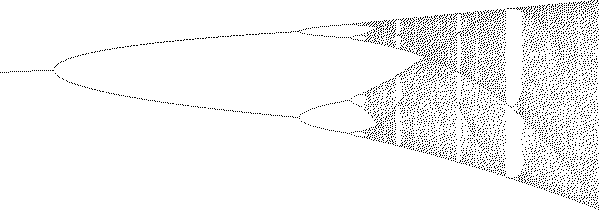
\includegraphics[width=3in]{figures/logistic-traditional-200.png}
\caption{A bifurcation diagram of the Logistic Map, rendered with 200 iterations per pixel column and traditional 1-bit point plotting.}
\end{figure}

\begin{figure}[htb]
\centering
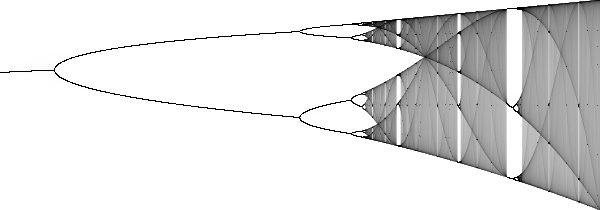
\includegraphics[width=3in]{figures/logistic-histogram-8m.png}
\caption{At the same image resolution, histogram-based rendering shows the extra detail obtained by running 8 million iterations per pixel column.}
\end{figure}

\end{subfigures}

As can be seen in figure \ref{logistic}, using a histogram exposes an enormous amount of
detail.  The image here is one of the canonical examples in nonlinear dynamics: a bifurcation
diagram of the \emph{logistic map}, an iterative equation for modelling animal populations.
Both images have a width of 600 pixels, but the 1-bit plot can only show approximately 200
points per column before things become too saturated to be useful.  In the histogram example
each column contains 8 million points.  While this is far beyond what can be displayed or
printed statically, the tone-mapping operator can be adjusted to expose different details
in the image.  The standard plotting technique here does not suffice to show the true structure
of this image;  one can see several horizontal rows of points with much higher density in
the histogram rendering, but these are completely hidden in the traditional plot.

\section{Related Work}
Tone mapping of high dynamic range images has been studied extensively, primarily in the
context of digital photography.  A comprehensive survey of tone-mapping techniques can be
found in \cite{kd}.  Some particularly influential tone-mapping operators are discussed
in \cite{jt}, \cite{jtjhbg} and \cite{gw}.

Histogram-based imaging techniques have been used previously in the rendering of so-called
``fractal flames.''  These are discussed in Scott Draves' informal paper describing the
internals of the \emph{Electric Sheep} screen-saver software\cite{sd}.

\section{Uniqueness of the Approach}
Because total histogram density is maintained during the computation run, the actual
tone-mapping step can be performed at any time.  This allows a low quality image to
be produced almost immediately, while further iterations merely add more detail.  Like
other techniques which progressively refine an image, this method performs particularly
well in interactive applications.  Iterations can be performed continuously in the
background while the tone-mapping stage is run repeatedly according to the rate at which
the histogram is changing.  It becomes computationally very cheap to change the system's
parameters, reset the histogram, and quickly obtain a low-quality rendering with the
new parameters.

This real-time potential has a profound impact on the way an artist or other user can
interact with the chaotic map's parameter space. \emph{Apophysis}\footnote{http://www.apophysis.org/}
is a tool for rendering fractal flames using the same histogram-based engine used by \emph{Electric Sheep}.
Despite this, its user interface fails to provide real-time feedback. Like other more traditional
fractal applications, it provides indirect ways to manipulate the parameter space. Perhaps the most
powerful of these indirect methods are \emph{mutations}, where the computer creates several versions
of an image, each with randomly perturbed parameters, then the user selects the one that most appeals
to them. The user closes a feedback loop which performs a hill-climbing optimization in order
to locally find the most pleasing parameter set for a fractal.

In order to take advantage of histogram-based rendering's real-time capabilities, our
\emph{Fyre}\footnote{http://fyre.navi.cx/} software takes this optimization strategy one step
further. The image updates in real-time, and various ``tools'' are provided that map mouse movements
to different aspects of the high-dimensional parameter space. This creates a strong coupling
between the user's hand movements and the perceived changes in rendering output. Rather than
selecting mutations at discrete intervals, the chaotic map becomes part of the user's motor control
feedback loop. With current input devices this restricts the user to explore two dimensions of the
parameter space at a time, but they have much better control over these dimensions. It is as if the
user can just grab hold of the parameters and move them in a solid way, making this hill-climbing
optimization process very intuitive.

This approach makes the algorithm particularly suitable to parallel processing.  If the
system being visualized converges toward a single attractor, many iteraton or integration
runs can be performed simultaneously.  Periodically, the histograms produced by each
of these can be merged.  This can dramatically improve the quality of images, and makes
this technique feasable even for slow computations and high-dimensional systems where a
plane of section is used to produce the image.

\section{Results}
By using histograms and high dynamic range imaging techniques, iterative systems can be
visualized in much higher detail than conventional plotting techniques.  Because
nonlinear iterative systems can exhibit such complexity in state space, a visualization
tool capable of showing long-term behavior is required. This technique has shown to
work particularly well in the visualization of strange attractors and other chaotic
systems.

The ability to explore parameter space interactively and create high-quality images
using the same algorithm is a very powerful tool.  In addition, because the tone-mapping
operator can be changed at any point, rendering controls such as exposure and color
interpolation can be adjusted in real time, even while computation continues. Depending
on the input system, the algorithm extends gracefully to parallel processing, making
it a feasable visualization technique even for extremely computationally intensive
systems.

\begin{thebibliography}{77}
\bibitem{kd} Devlin, Kate: ``A Review of Tone Reproduction Techniques'' {\it Technical Report CSTR-02-005,} Department of Computer Science, University of Bristol, November 2002.
\bibitem{sd} Draves, Scott: ``The Fractal Flame Algorithm.'' Available online, http://flam3.com/flame.pdf
% \bibitem{fdjd} Durand, F. and J. Dorsey: ``Interactive Tone Mapping,'' {\it Rendering Techniques 2000: 11th Eurographics Workshop on Rendering,} pp. 219-230, Eurographics, June 2000. ISBN 3-211-83535.
\bibitem{jt} Tumblin, Jack: {\it Three Methods of Detail-Preserving Contrast Reduction for Displayed Images.} Phd thesis, Georgia Institute of Technology, December 1999.
\bibitem{jtjhbg} Tumblin, J., J.K. Hodgins and B.K. Guenter: ``Two Methods for Display of High Contrast Images.'' {\it ACM Transactions on Graphics,} 18(1):56-94, January 1999, ISSN 0730-0301.
\bibitem{gw} Ward, Gregory: ``High dynamic range imaging,'' In {\it Proceedings of the Ninth Colour Imaging Conference,} November 2001.
\end{thebibliography}

\end{document}
